\documentclass[11pt]{article}
\usepackage[letterpaper]{geometry}
\usepackage{MATH561}
\usepackage{SetTheory}

\begin{document}
\noindent \textbf{\Large{Caleb Logemann \\
MATH 561 Numerical Analysis I \\
Homework 2
}}

\begin{enumerate}
    \item[\#1] % #1 done
        \begin{enumerate}
            \item[(a)] \hfill \\
                \begin{center}
                    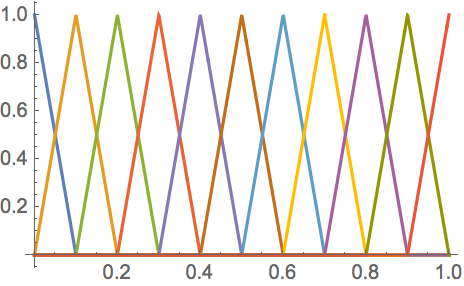
\includegraphics[scale=.5]{Figures/02_1a.png}
                \end{center}

            \item[(b)]
                If $j = k$, then $\pi_j\p{k/n} = \pi_j{j/n} = 1$.
                If $j \neq k$, then $\pi_j\p{k/n} = 0$, because $k/n$ is
                outside of the division that is the support of $\pi_j$

            \item[(c)]
                Let $c_0, c_1, \ldots, c_n \in \RR$ be given such that
                $\sum{i=0}{n}{c_i \pi_i\p{t}} = 0$ for all $t \in \p{0,1}$
                Consider $t = k/n$ for some $k \in \set{0, 1, \ldots, n}$, then
                $\sum{i=0}{n}{c_i \pi_i\p{k/n}} = c_k \pi_k\p{k/n}$, because
                $\pi_j{k/n} = 0$ for all $j \neq k$.
                Also $\pi_k\p{k/n} = 1$, so $c_k \pi_k\p{k/n} = c_k$.
                However this sum must be equal to $0$ at $t = k/n$, so $c_k = 0$.
                This implies that $c_0 = c_1 = \cdots = c_n = 0$.
                Thus the $\set{\pi_j}_{j=0}^n$ is linearly independent over the
                interval $(0, 1)$.
                This also implies that $\set{\pi_j}_{j=0}^n$ is linearly independent
                over the points $\set{0, 1/n, \ldots, \frac{n-1}{n}, 1}$, because
                at these points only one of the functions contributes to the
                overall sum.

            \item[(d)]
                For $\abs{i - j} > 1$, $\pi_i(t) \pi_j(t) = 0$ for $t \in (0, 1)$.
                Therefore $\dintt{0}{1}{\pi_i(t) \pi_j(t)}{t} = 0$ and $a_{ij} = 0$
                for $\abs{i - j} > 1$.

                For $\abs{i - j} = 1$, without loss of generality assume $j = i + 1$.
                Note that $\supp\p{\pi_i(t)\pi_j(t)} = (i/n, i+1/n) = (i/n, j/n)$
                \begin{align*}
                    \dintt{0}{1}{\pi_i(t)\pi_j(t)}{t} &= \dintt{0}{1}{\pi_i(t)\pi_{i+1}(t)}{t}
                    \intertext{Since $\supp\p{\pi_i(t)\pi_{i+1}(t)} = (i/n, i+1/n)$}
                    &= \dintt{i/n}{\p{i+1}/n}{\pi_i(t)\pi_{i+1}(t)}{t}
                    \intertext{On this interval $\pi_i(t) = -nt + i + 1$ and $\pi_{i+1}(t) = nt - i$}
                    &= \dintt{i/n}{\p{i+1}/n}{\p{-nt + i + 1}\p{nt - i}}{t} \\
                    &= \dintt{i/n}{\p{i+1}/n}{-n^2t^2 + int + int + nt - i^2 - i}{t} \\
                    &= \dintt{i/n}{\p{i+1}/n}{-n^2t^2 + (2i+1)nt - i^2 - i}{t} \\
                    &= \eval{-\frac{n^2}{3}t^3 + \frac{(2i+1)n}{2}t^2 - (i^2 + i)t}{t=i/n}{\p{i+1}/n} \\
                    &= \eval{-\frac{n^2}{3}t^3 + \frac{(2i+1)n}{2}t^2 - (i^2 + i)t}{t=i/n}{\p{i+1}/n} \\
                    &= -\frac{n^2}{3}\p{\frac{i+1}{n}}^3 + \frac{(2i+1)n}{2}\p{\frac{i+1}{n}}^2 - (i^2 + i)\frac{i+1}{n} \\
                    &+ \frac{n^2}{3}\p{\frac{i}{n}}^3 - \frac{(2i+1)n}{2}\p{\frac{i}{n}}^2 + (i^2 + i)\frac{i}{n} \\
                    &= -\frac{(i+1)^3}{3n} + \frac{(2i+1)(i+1)^2}{2n} - \frac{(i^2 + i)(i+1)}{n} + \frac{i^3}{3n} - \frac{(2i+1)i^2}{2n} + \frac{i^3 + i^2}{n} \\
                    &= -\frac{3i^2 + 3i + 1}{3n} + \frac{(2i+1)^2}{2n} - \frac{(i^2 + i)}{n} \\
                    &= \frac{1}{6n}
                \end{align*}

                For $\abs{i - j} = 0$, that is $i = j$.
                Note that $\supp\p{\pi_i(t)^2} = (i-1/n, i+1/n)$.
                \begin{align*}
                    \dintt{0}{1}{\pi_i(t)^2}{t} &= \dintt{(i-1)/n}{(i+1)/n}{\pi_i(t)^2}{t}
                    \intertext{This can be split into two subintervals}
                    &= \dintt{(i-1)/n}{i/n}{\pi_i(t)^2}{t} + \dintt{i/n}{(i+1)/n}{\pi_i(t)^2}{t}
                    \intertext{On $((i-1)/n, i)$, $\pi_i(t) = nt - i + 1$ and on $(i/n, (i+1)/n$, $\pi_i(t) = -nt + i + 1$}
                    &= \dintt{(i-1)/n}{i/n}{(nt - i + 1)^2}{t} + \dintt{i/n}{(i+1)/n}{(-nt + i + 1)^2}{t}
                    \intertext{Because of symmetry}
                    &= 2\dintt{(i-1)/n}{i/n}{n^2t^2 - 2n(i-1)t + (i-1)^2}{t} \\
                    &= \eval{2\p{\frac{n^2}{3} t^3 - n(i-1) t^2 + (i-1)^2t}}{t = (i-1)/n}{i/n} \\
                    &= 2\p{\frac{i^3}{3n} - \frac{i^3-i^2}{n} + \frac{i(i-1)^2}{n} - \frac{(i-1)^3}{3n} + \frac{(i-1)^3}{n} - \frac{(i-1)^3}{n}} \\
                    &= 2\p{\frac{-i^2 + i}{n} + \frac{3i^2 - 3i + 1}{3n}} \\
                    &= \frac{2}{3n}
                \end{align*}
                If $i = j = 0$ or $i = j = n$, then symmetry does not apply, that is there is no other half.
                So $a_{00} = a_{nn}= \frac{1}{2} a_{ii} = \frac{1}{3n}$ for $1 \le i \le n-1$.
                Therefore
                \begin{align*}
                    a_{ij} = \begin{dcases}
                        0 & \abs{i - j} > 1 \\
                        \frac{1}{6n} & \abs{i - j} = 1 \\
                        \frac{2}{3n} & \abs{i - j} = 0\text{ and }1 \le i \le n-1 \\
                        \frac{1}{3n} & i = j = 0\text{ or }i = j = n
                    \end{dcases}
                \end{align*}
        \end{enumerate}

    \item[\#2] % #2 finding upper bounds for error
        \begin{enumerate}
            \item[(a)]
                Find an upper bound for $\norm[\infty]{f - p_2(f; \cdot)}$ on
                equally spaced points.
                By the error of the interpolation problem $f(x) - p_2(f;x) =
                (x - x_0)(x - x_1)(x - x_2) \frac{f'''(\xi)}{6}$
                Thus $\norm[\infty]{f - p_2(f; \cdot)} =
                \norm[\infty]{(x - x_0)(x - x_1)(x - x_2)}
                \frac{\norm[\infty]{f'''(x)}}{6}$.
                Using calculus, $\norm[\infty]{(x - x_0)(x - x_1)(x - x_2)}$ can be found.
                \begin{align*}
                    g(x) &= (x - x_0)(x - x_1)(x - x_2) \\
                    g'(x)&= (x - x_1)(x - x_2) + (x - x_0)(x - x_2) + (x - x_0)(x - x_1) \\
                         &= 3x^2 - 2(x_0 + x_1 + x_2)x + x_0x_1 + x_0x_2 + x_1x_2 \\
                         &= 3x^2 - 6(x_0 + h)x + 3x_0^2 + 6hx_0 + 2h^2
                    \intertext{Using the quadractic formula to solve for when $g'(x) = 0$}
                    x &= \frac{6(x_0 + h) \pm \sqrt{36(x_0 + h)^2 - 4\cdot3(3x_0^2 + 6hx_0 + 2h^2)}}{6} \\
                      &= \frac{6(x_0 + h) \pm 2\sqrt{3\p{3(x_0 + h)^2 - (3x_0^2 + 6hx_0 + 2h^2)}}}{6} \\
                      &= \frac{3(x_0 + h) \pm \sqrt{3\p{3x_0^2 + 6hx_0 + 3h^2 - (3x_0^2 + 6hx_0 + 2h^2)}}}{3} \\
                      &= \frac{3(x_0 + h) \pm \sqrt{3h^2}}{3} \\
                      &= x_1 \pm \frac{\sqrt{3}}{3}h
                \end{align*}
                So $g(x)$ achieves its maximum at $x = x_1 \pm \frac{\sqrt{3}}{3}h$.
                So $\abs{g(x)} \le g(x_1 + \frac{\sqrt{3}}{3}h)$.
                \begin{align*}
                    g(x_1 - \frac{\sqrt{3}}{3}h) &= (x_1 - \frac{\sqrt{3}}{3}h - x_0)(x_1 - \frac{\sqrt{3}}{3}h - x_1)(x_1 - \frac{\sqrt{3}}{3}h - x_2) \\
                    &= \frac{3 - \sqrt{3}}{3}h \times \frac{-\sqrt{3}}{3}h \times \frac{-\sqrt{3} - 3}{3}(h) \\
                    &= \frac{-3\sqrt{3} + 3}{9}h^2 \times \frac{-\sqrt{3} - 3}{3}(h) \\
                    &= \frac{6\sqrt{3}}{27} h^3 \\
                    &= \frac{2\sqrt{3}}{9} h^3
                \end{align*}
                Therefore $\norm[\infty]{f - p_2(f; \cdot)} = \frac{2\sqrt{3}}{9} h^3
                \frac{\norm[\infty]{f'''(x)}}{6} = \frac{1}{9\sqrt{3}} \norm[\infty]{f'''(x)} h^3$.

            \item[(b)]
                Let $t_0, t_1, t_2$ be the Chebyshev nodes on $[-1, 1]$.
                Then we know that $t_i = \cos{\frac{2i + 1}{6}\pi}$, so
                $t_0 = \cos(\pi/6) = \sqrt{3}/2$, $t_1 = \cos(\pi/2) = 0$ and
                $\cos(5\pi/6) = -\sqrt{3}/2$.
                In order to interpolate on $[x_0, x_2]$, these nodes need to be
                mapped to that domain.
                Let the map be $x = x_1 + ht$.
                The $c_0 = x_1 + \sqrt{3}/2 h, c_1 = x_1, c_2 = x_1 - \sqrt{3}/2 h$,
                will be the Chebyshev nodes on $[x_0, x_2]$.

                Then we know that the error will be $f(x) - p_2(f;x) =
                (x - c_0)(x - c_1)(x - c_2) \frac{f'''(\xi)}{6}$.
                \begin{align*}
                    (x - c_0)(x - c_1)(x - c_2) &= (x - (x_1 + \sqrt{3}/2 h))(x - x_1)(x - (x_1 - \sqrt{3}/2 h) \\
                                                &= (t - t_0)h(t-t_1)h(t - t_2)h \\
                                                &= \frac{1}{4} T_2(t) h^3 \\
                \end{align*}
                Therefore $\norm[\infty]{f(x) - p_2(f;x)} = \frac{1}{4} h^3 \frac{\norm[\infty]{f'''(x)}}{6} =
                \frac{1}{24} \norm[\infty]{f'''(x)} h^3$.
                This is a much better bound than for the equally spaced nodes.
        \end{enumerate}

    \item[\#4] % #4
    \item[\#6] % #6
        \begin{enumerate}
            \item[(a)]
                Table of divided differences \hfill \\
                \begin{tabular}{cccccc}
                    $x_i$ & $f_i$ &    &    &    &    \\
                    \midrule
                       -1 &     0 &    &    &    &    \\
                       -1 &     0 &  0 &    &    &    \\
                        0 &     1 &  1 &  1 &    &    \\
                        1 &     0 & -1 & -1 & -1 &    \\
                        1 &     0 &  0 &  1 &  1 &  1 \\
                \end{tabular}

                Using this table of divided differences the Hermite
                interpolation polynomial is $p(x) = (x + 1)^2 - (x + 1)^2 x +
                (x + 1)^2 x (x - 1)$.
                This can be simplified to $p(x) = x^4 - 2x^2 + 1$.

            \item[(b)]
                \begin{enumerate}
                    \item[(b.1)]
                        The error can be expressed as $e(x) = f(x) - p(x) =
                        (x + 1)^2 x (x-1)^2 \frac{f^{(5)}(\xi)}{5!}$ for $x
                        \in \br{-1, 1}$.
                        This can be simplified by noting that $(x + 1)(x - 1) = (x^2 - 1)$.
                        Therefore $e(x) = x(x^2-1)^2 \frac{f^{(5)}(\xi)}{5!}$

                    \item[(b.2)]
                        This can be bounded on $x \in \br{-1, 1}$ by noting that
                        $f^{(5)}(x) = -\frac{1}{2} \pi^5 \sin{\pi x}$.
                        Therefore $\abs{f^{(5)}(\xi)} \le \frac{\pi^5}{2}$.
                        So $\abs{e(x)} \le \abs{x(x^2-1)^2 \frac{\pi^5}{2\cdot5!}}$

                    \item[(b.3)]
                        Consider $g(x) = x(x^2 - 1)^2$, where does this
                        achieve its maxima on $\br{-1, 1}$.
                        These maxima can be found using calculus.
                        \begin{align*}
                            g'(x) &= 2x(x^2 - 1)2x + (x^2 - 1)^2 \\
                                  &= (x^2 - 1)(4x^2 + x^2 - 1) \\
                                  &= (x^2 - 1)(5x^2 - 1) \\
                        \end{align*}
                        Therefore $g'(x) = 0$ at $x = 1, -1, 
                        \frac{1}{\sqrt{5}}, \frac{1}{\sqrt{5}}$.
                        Since $g(1) = 0$ and $g(-1) = 0$, these are not maxima.
                        However $g(\pm \frac{1}{\sqrt{5}}) = \pm\frac{1}{\sqrt{5}} \frac{16}{25}$
                        are relative extrema.
                        So $g(\frac{1}{\sqrt{5}}) = \frac{16}{25\sqrt{5}}$ is
                        the maximum on $\br{-1,1}$.
                        Thus $\max_{-1 \le x \le 1}\p{e(x)} \le
                        \frac{16}{25\sqrt{5}} \frac{\pi^5}{2\cdot5!} \approx .36495$
                \end{enumerate}
        \end{enumerate}

    \item[\#8] % #8
        \begin{enumerate}
            \item[(a)] Code for solving a tridiagonal system using Gaussian Elimination
                \lstinputlisting[language=Matlab]{../+NumericalAnalysis/tridiag.m}
            \item[(b)] Code for creating natural cubic spline and displaying errormax
                \lstinputlisting[language=Matlab]{../+NumericalAnalysis/cubicSpline.m}
                \lstinputlisting[language=Matlab]{H02.m}
            \item[(c)]
        \begin{verbatim}
>> H02
part (1)
e^(-x)
       1   4.9030e-04
       2   1.3163e-04
       3   3.5026e-05
       4   9.5467e-06
       5   2.2047e-06
       6   4.2094e-07
       7   3.4559e-06
       8   1.2809e-05
       9   4.8441e-05
      10   1.8036e-04
x^(5/2)
       1   2.0524e-04
       2   5.3392e-05
       3   1.6192e-05
       4   2.7607e-06
       5   1.2880e-06
       6   9.8059e-06
       7   3.4951e-05
       8   1.3252e-04
       9   4.9310e-04
      10   1.8416e-03
part (2)
x^(5/2)
       1   6.6901e-07
       2   2.3550e-07
       3   1.1749e-06
       4   1.6950e-06
       5   1.5853e-06
       6   1.6441e-05
       7   6.8027e-05
       8   3.2950e-04
       9   1.4755e-03
      10   6.5448e-03
        \end{verbatim}
        This output shows the maximum error of these spline interpolations.
        The maximum error shows how the natural cubic spline interpolates
        better on the inner subdivisions.
        The natural cubic spline has larger errors near the endpoints, because
        the second derivative is forced to be zero at the endpoints.
        Note in part two because the subdivisions are no longer equal, the
        interpolation is better at the beggining where the subdivisions are smaller.
        \end{enumerate}
\end{enumerate}
\end{document}
